\section{Consultation de documents}
\label{sec:consultation}

La page de consultation de documents est une page générique devant proposer trois modes de consultation :
\begin{itemize}
\item Article
\item Journal
\item Revue de presse
\end{itemize}

Il est important d’apporter une valeur ajoutée à cette consultation de document. Trois objectifs ont donc été définis :
\begin{itemize}
\item Informer : informer l’utilisateur sur le document qu’il consulte
\item Consulter : permettre à l’utilisateur de consulter le document
\item Guider : guider l’utilisateur en lui proposant de consulter d’autres documents
\end{itemize}
C’est selon ces trois objectifs que l’interface et les fonctionnalités ont été imaginées.


\subsection{Informer}
\label{sec:consultation_informer}
	La consultation d’un document ne doit pas se cantonner à un simple affichage d’image. Il est également important d’informer l’utilisateur sur ce qu’il consulte. La partie gauche de la page y sera dédiée. Celle-ci sera rétractable afin de laisser à la visionneuse d'image plus de place sur la page quand l'utilisateur n'a pas besoin de ces informations.
On y trouvera des informations concernant :
\begin{itemize}
\item Le journal en cours de consultation : titre, date.
\item L’article en cours de consultation : titre, tags.
\end{itemize}
\bigskip
\par
	Cette liste d’information n’est pas exhaustive, elle dépendra des métadonnées qui nous seront mises à disposition.
	L’utilisateur pourra également être acteur de la classification des articles. En effet, l'utilisateur pourra aussi ajouter des tags. En effet, lorsque celui-ci sélectionne un article, il aura alors la possibilité d'y ajouter des tags. À la manière de twitter, la saisie de tags sera facilité grâce à de l'auto-complétion afin de ne pas avoir plusieurs tags similaire ayant différents orthographes dans la base de données. Il lui sera aussi possible d’ajouter l’article à une revue de presse ou à ses favoris. Il pourra alors choisir une revue de presse en effectuant une recherche ; les revues de presse qu’il a créées ou celles auxquelles il a participé seront proposées en premier dans les résultats de recherche. S’il ne trouve pas la revue de presse qui lui convient, l’utilisateur aura la possibilité d’en créer une (voir maquette en bas à gauche). 

\subsection{Consulter}
\label{sec:consultation_consulter}
La fonctionnalité principale est bien sûr de consulter des documents. Le milieu de la page y sera consacré.
L’interface de visualisation affichera une page de journal avec un focus différent selon le mode de lecture :
\begin{itemize}
\item “Article” et “Revue de presse” : la visionneuse zoome sur l’article concerné. Celui-ci sera mis en évidence par un calque transparent coloré.
\item “Journal” : la visionneuse affiche la première page du journal, sans zoom.
\end{itemize}
\bigskip
\par
Si l’utilisateur survole un autre article, celui-ci sera également mis en évidence par un calque.
	L’utilisateur aura aussi la possibilité de zoomer/dézoomer et de se déplacer dans la page, ainsi que d’effectuer une recherche textuelle dans la page. Pour avoir une utilisation plus fluide, l'utilisateur pourra double cliquer sur un article, et ce afin de zoomer directement sur ce dernier. Double cliquer à nouveau dessus réinitalisera le zoom afin d'avoir à nouveau la page d'ensemble. Si la lecture est en mode “Revue de presse”, il sera possible de passer à l’article précédent ou suivant de la revue de presse. Dans tous les cas, l'utilisateur pourra naviguer entre toutes les pages du journal.

\subsection{Guider}
\label{sec:consultation_guider}

	Tous les utilisateurs ne viendront pas en sachant quel article ils souhaitent consulter; beaucoup d’entre eux voudront simplement découvrir. Dans cette mesure, il semble important de guider l’utilisateur. La partie droite de la page y sera consacrée. Par ailleurs, cette espace permettra aussi à l'utilisateur de découvrir l'architecture de la page qu'il est en train de lire; il pourra ainsi voir la liste des articles contenus dans la page. En cliquant sur un article, celui-ci sera mis en évidence sur la page grâce à un calque transparent coloré.

	Trois fonctionnalités participeront à ce guidage :
\begin{itemize}
\item Articles similaires : une sélection d’articles similaires à celui en cours de lecture sera proposée à l’utilisateur. Ces recommandations pourront s’effectuer selon plusieurs critères : ressemblances de mots, journaux, périodes ou tags identiques.
\item Revues de presses associées : une liste des revues de presse contenant l’article en cours de visualisation sera proposée à l’utilisateur. L’idée est de le diriger vers des thématiques pouvant potentiellement l’intéresser.
\item Articles de la revue de presse : si la lecture est en mode “Revue de presse”, l’utilisateur aura accès à la liste des articles de celle-ci.
\end{itemize}

\bigskip

    \begin{figure}[H]
        \centering
        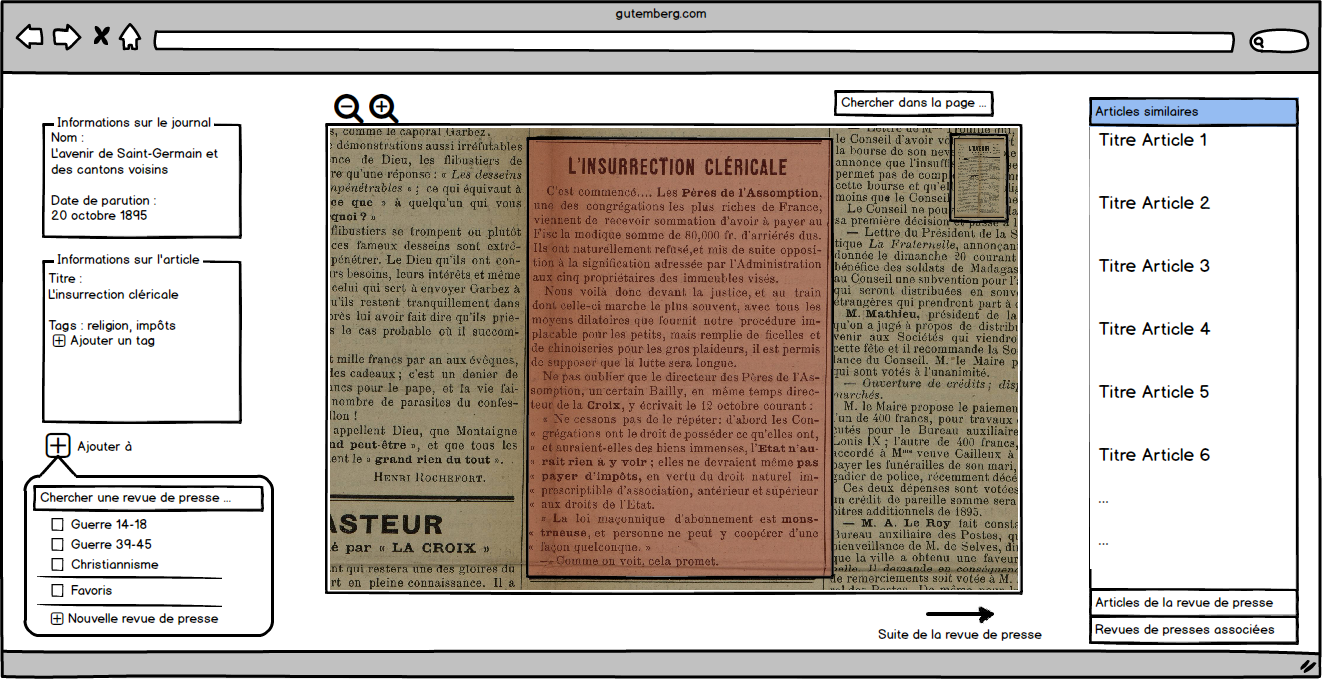
\includegraphics[width=\textwidth]{figures/consultation.png}
            \caption{Page de consultation de documents}
            \label{fig:consultation}
    \end{figure}